\chapter{Introduction}
\label{chapter:introduction} %%%%%%%%%%%%%%%%%%%%%%%%%%%%
%\section{Introduction}
\section{Introduction}
\label{sec:intro}


\section{Background}
\label{sec:background}


\section{Problem Statement} \label{problem}


\section{Objectives} \label{researchobjectives}
\subsection{Main Objective }
\noindent The main objective is...

\subsection{Specific Objectives}
\begin{enumerate}[(i)]
\item To review...
\item To develop...
\item To test...
\end{enumerate}
%\newpage
\section{Research Questions} \label{researchquestions}
\begin{enumerate}[(i)]
\item What are...
\item What are...
\item How best...
\end{enumerate}
\section{Project Significance} \label{researchsignificance}
\subsection{Value Proposition}

\subsection{Innovation}

\subsection{Impact}

\subsection{Business Component}

%\newpage
\section{Scope of the Study}
\noindent The study will be carried out...
%\newpage

%%%%%%%%%%%%%%%%%%%%%%%%%%%%% Literature Review Section%%%%%%%%%%%%%%%%%%%%%%%%%%%%%%%%%%%%%%
\chapter{Literature Review}\label{chapter:Literature_Review}
\section{Literature Review}
In this section, we present the findings from several literal sources with regard to the major concepts associated with this research. Information obtained from several journal articles, conference papers, relevant workshops, reputable websites, and published books are compiled to provide theoretical grounding and practical justification for the problem under investigation.

\section{...}


\section{...}

\section{...}

\chapter{Methodology}\label{chapter:Methodology}
\section{Methodology Name/Overview}

%\begin{figure}
 %   \centering
  %  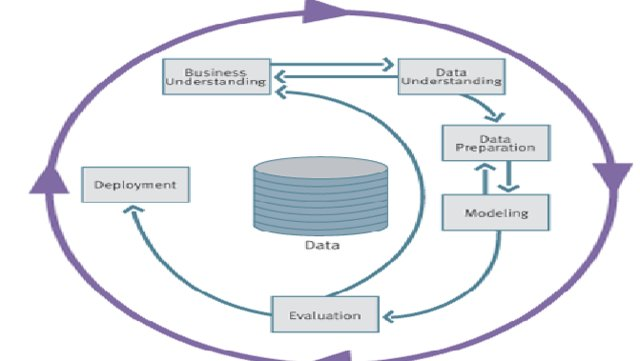
\includegraphics{images/crispdm.jpg}
   % \caption{CRISP-DM Methodology}
    %\label{fig:my_label}
%\end{figure}

\section{...}

%\newpage

\section{...}

\subsection{...}

\subsection{...}

\chapter{Data Representation, Analysis and Interpretation}\label{chapter:Results}
\section{...}

\section{...}

\chapter{System Development and Implementation}\label{chapter:System}
\section{Introduction}
This chapter has information on the implementation of the project. It identifies the user and system requirements, and specifications of the system.

\section{Requirements Identified}


\subsection{User Requirements}

\subsubsection{Other User Requirements}


\subsection{Functional Requirements}


\subsection{Non-Functional Requirements}

\subsubsection{Security}


\subsubsection{Performance}


\subsubsection{Usability}


\subsubsection{Scalability}


\subsection{System Requirements}


\subsubsection{Hardware Specification}
The following hardware specifications were used because they are the least affordable and the system has been tested on them as per the results in the data output section. The specifications are shown in the table below;\\

\begin{tabularx}{0.8\textwidth} { 
  | >{\raggedright\arraybackslash}X 
  | >{\raggedright\arraybackslash}X | }
 \hline
 Hardware  & Minimum System Requirements \\
 \hline
 Processor  & Intel Duo Core 2.0 GHz  \\
 \hline
 Memory  & 512 MB RAM \\
 \hline
 Hard Disk Space  & 40 GB  \\
 \hline
\end{tabularx}

\subsubsection{Software Specification}
The table below shows the software specifications needed for this system;

\begin{tabularx}{0.8\textwidth} { 
  | >{\raggedright\arraybackslash}X 
  | >{\raggedright\arraybackslash}X | }
 \hline
 Software  & Minimum System Requirements \\
 \hline
 Operating System  & Windows 7/8/10, Linux  \\
 \hline
 Database  & SQLite3 \\
 \hline
 Languages  & Python (Django), JavaScript \\
 \hline
\end{tabularx}

\subsubsection{Languages Used}


\section{System Flow}

\subsection{System Flow Chart}


\subsection{Use Case Diagram}

\section{User Interfaces}

\chapter{Discussion}\label{chapter:Discuss}
\section{Research Overview}


\section{Conclusion}

\section{Recommendation}


\section{Future Work}


%%%%%%%%%%%%%%%%%%%% End of conclusion %%%%%%%%%%%%%%%%%%%%%%%%%%%%